\documentclass[11pt]{article}
\usepackage[utf8x]{inputenc}
\usepackage{amsmath}
\usepackage{graphicx}
\usepackage{float}
\usepackage{array}
\usepackage{dsfont}
\usepackage{amsfonts}
\usepackage{lipsum}
\usepackage{enumitem}
\usepackage{epstopdf}
\usepackage[T1]{fontenc}
\usepackage[colorinlistoftodos]{todonotes}
\usepackage[left=2cm,right= 2cm,top=3cm,bottom=2.5cm,a4paper]{geometry}
\usepackage{listings}
\usepackage{minted}
\usepackage{multicol}
\usepackage{fancyhdr}
\usepackage{caption}
\usepackage{cite}
\usepackage{cleveref}
\usepackage{siunitx}
\setlength{\columnsep}{1cm}
\setlength{\parindent}{0pt}
\newcommand{\deriv}{\mathrm{d}}
\usepackage{color}  
\usepackage{hyperref}
\hypersetup{
    colorlinks=true, 
    linktoc=all,    
    linkcolor=black,
    citecolor=black,
}
\lstset{
    language=R,
    basicstyle=\scriptsize\ttfamily,
    commentstyle=\ttfamily\color{red},
    numbers=left,
    numberstyle=\ttfamily\color{blue}\footnotesize,
    stepnumber=1,
    numbersep=5pt,
    backgroundcolor=\color{white},
    showspaces=false,
    showstringspaces=false,
    showtabs=false,
    frame=single,
    tabsize=2,
    captionpos=b,
    breaklines=true,
    breakatwhitespace=false,
    title=\lstname,
    escapeinside={},
    keywordstyle={},
    morekeywords={}
}

\pagestyle{fancy}
\fancyhf{}
\rhead{PH370 Physics Labs}
\lhead{LLR.2 - Stress \& Strain}
\rfoot{-\thepage\centering-}

\begin{document}
\begin{titlepage}

\newgeometry{left=1.5in,right=1.5in,top=2.5in,bottom=2.5in}
\newcommand{\HRule}{\rule{\linewidth}{0.5mm}}

\begin{centering} 
 
%------------------------------------------------------------------------
%	HEADING SECTIONS
%------------------------------------------------------------------------


\includegraphics[scale=0.4]{Uni_of_Kent_Logo.png}\\[1cm]

%------------------------------------------------------------------------
%	TITLE SECTION
%------------------------------------------------------------------------

\HRule \\[0.4cm]
\textsc{\large Astronomy, Space Science and Astrophysics}\\[0.4cm]
{\huge \bfseries Stress \& Strain}\\[0.4cm]
\HRule \\[1.0cm]

%------------------------------------------------------------------------
%	DATE SECTION
%------------------------------------------------------------------------

\textsc{\Large Stage 1 - PH370 Physics Labs}\\[0.5cm] 
{\large Monday 12th/19th February 2018}\\[1.0cm]

%------------------------------------------------------------------------
%	AUTHOR SECTION
%------------------------------------------------------------------------

\begin{minipage}{0.625\textwidth}
\centering

\emph{\large Report Author:} \large Lukasz R Tomaszewski \\ [0.2cm]
\emph{\large Lab Partner:} \large Joshua F Young \\
\emph{\large Lab Partner:} \large Benedict J Wye \\

\end{minipage}\\[2cm]

\vfill
\end{centering} 
\end{titlepage}

%------------------------------------------------------------------------
%------------------------------------------------------------------------
%	CONTENTS  
%------------------------------------------------------------------------
%------------------------------------------------------------------------

\newpage
\begin{titlepage}
\begin{tableofcontents}

\end{tableofcontents}
\end{titlepage}

%-----------------------------------------------------------------------
%-----------------------------------------------------------------------
%	INTRODUCTION
%-----------------------------------------------------------------------
%-----------------------------------------------------------------------

\begin{multicols}{2}

\section{Introduction}
\label{Introduction Section}

The purpose of this experiment is to test and measure multiple quantities listed in \href{Data Collected SubSection} in 4 materials listed in \href{Apparatus SubSection}. Each material will be tested to destruction first then tested to their individual yield points, which will allow for the Young's modulus to be found and each materials tensile stress, strain and yield stress. The purpose is to understand why certain materials are better suited for different purposes.

%-----------------------------------------------------------------------
%-----------------------------------------------------------------------
%	AIMS & EQUIPMENT
%-----------------------------------------------------------------------
%-----------------------------------------------------------------------

\section{Aims \& Equipment}
\label{AimsEquipmentSection}

%-----------------------------------------------------------------------
%	APPARTUS
%-----------------------------------------------------------------------

\subsection{Apparatus}
\label{Apparatus SubSection}

\begin{itemize}
    \item{x4 Strips of mild steel}
    \item{x4 Strips of duralumin}
    \item{x4 Strips of aluminium}
    \item{x4 Strips of PVC}
    \item{x1 Mini tensile tester}
    \item{x1 Vernier caliper}
\end{itemize}

%-----------------------------------------------------------------------
%	DATA COLLECTED
%-----------------------------------------------------------------------

\subsection{Data Collected}
\label{Data Collected SubSection}

\begin{itemize}
    \item{Tensile stress of each material}
    \item{Tensile strain of each material}
    \item{Percentage elongation of each material}
    \item{Young's modulus of each material}
\end{itemize}

%-----------------------------------------------------------------------
%	RISK ASSESSMENT
%-----------------------------------------------------------------------

\subsection{Risk Assessment}
\label{Risk Assessment SubSection}

As this experiment involves testing samples of materials to destruction, the materials may splinter and become shrapnel which has the potential to cause physical damage to the operators hands/eyes and or any exposed upper body part. A guard will be used to keep the tested samples contained to stop shrapnel from causing harm to the operators, the guard is locked onto the test rig itself as an extra precaution. The materials \& equipment can fall off the edges of the desk and inflict bruising or injury to the operators feet or any lower body part, this will be controlled by keeping all the equipment in the centre of the desk and away from the edges of the desk.

%-----------------------------------------------------------------------
%-----------------------------------------------------------------------
%	EXPERIMENTAL PROCEDURE
%-----------------------------------------------------------------------
%-----------------------------------------------------------------------

\section{Experimental Procedure}
\label{Experimental Procedure Section}

%-----------------------------------------------------------------------
%	EXPERIMENT THEORY
%-----------------------------------------------------------------------

\subsection{Experiment Theory}
\label{Experiment Theory SubSection}

Hooke's Law specifies that the strain in a material is directly proportional to the applied stress within the materials elastic limit. When a majority of solid materials are subject to tensile stresses, within the materials specific elastic limit will obey Hooke's law;

\begin{equation} \label{Distance parallel to our line of sight equation}
{F = kx}
\end{equation}

\begin{equation*}
\begin{split}
&\text{Where;} \\
&\text{F = Force} \\
&\text{k = Spring constant} \\
&\text{x = Length of extension/compression} \\
\end{split}
\end{equation*}\\

Young's Modulus is a quantitative measure of the materials elasticity and or stiffness.

\begin{equation} \label{Distance parallel to our line of sight equation}
{E = \dfrac{Stress}{Strain}}
\end{equation}

\begin{equation*}
\begin{split}
&\text{Where;} \\
&\text{E = Young's Modulus} \\
&\text{Stress = Force per unit area} \\
&\text{Strain = extension/length} \\
\end{split}
\end{equation*}\\

\begin{figure}[H]
\centering
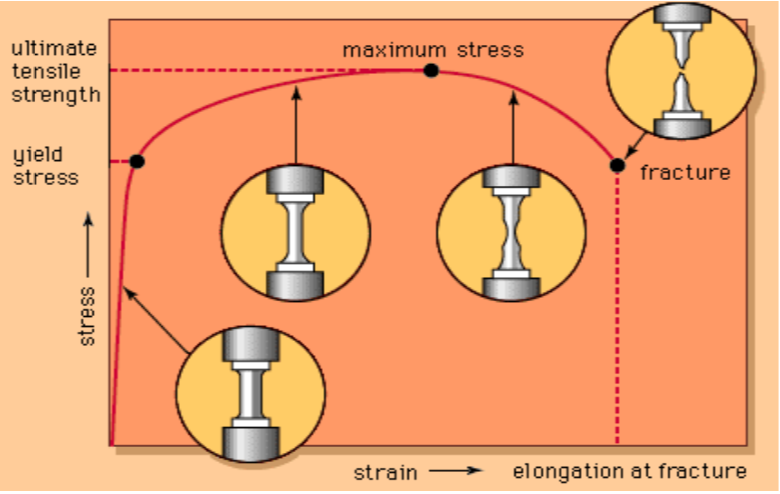
\includegraphics[scale=0.55]{Images/Behaviour_of_Extension.png}
\caption{Behaviour of Extension.}
\label{Behaviour_of_Extension}
\end{figure}

The diagram above found in \cite{LLR.2-2018} is a graph showing a material being stretched or compressed and what happens to the material during the its test duration, the resulting graph from this experiment should be similar to this.

%-----------------------------------------------------------------------
%	EXPERIMENTAL METHOD
%-----------------------------------------------------------------------

\subsection{Experimental Method}
\label{Experimental Method SubSection}

In the first stage of this experiment was to test each four materials to destruction by stretching them past their yield points unto their fracture point as figure \ref{Behaviour_of_Extension} shows. After the fracture point has been reached then another new piece of the same four materials will be tested individually and pushed only to their yield point. Using the data, the graph will be plotted found in section \ref{Main Results SubSection}. \\

Using the graphs, the yield point, tensile stress/ strain can be found and calculate the percentage of elongation, this allows for further analysis of the data and to prove the hypothesis of why certain materials are better than other in certain job requirements.

%-----------------------------------------------------------------------
%-----------------------------------------------------------------------
%	RESULT & DISSCUSSION
%-----------------------------------------------------------------------
%-----------------------------------------------------------------------

\section{Results \& Discussion}
\label{Results Discussion Section}

%-----------------------------------------------------------------------
%	MAIN RESULTS
%-----------------------------------------------------------------------

\subsection{Main Results}
\label{Main Results SubSection}

Aircraft fuselage are made of duralumin rather than aluminium due to the superior mechanical properties that duralumin has over aluminium. Duralumin is stronger and the same physical weight as aluminum which is imperative for an aircrafts fuselage which is exposed to harsh environmental effects. Even though it is an alloy of aluminium consisting of 94\% aluminium, its surface is a thin layer of aluminium which gives duralumin its extensive corrosion resistance. This will be proved throughout the experiment.\\

The materials used in this experiment were in bag labeled as the following; 

\begin{enumerate}[label=(Bag \Alph*)]
\centering
	\item{= (x4) PVC}
	\item{= (x4) Mild Steel}
    \item{= (x4) Aluminium}
    \item{= (x4) Duralumin}
\end{enumerate}

%-----------------------------------------------------------------------
%	PVC
%-----------------------------------------------------------------------

\subsection{PVC Sample}
\label{PVC Sample SubSection}

Using the mini tensile tester, two pieces of PVC strips were fitted and secured into the rig, 

\begin{figure}[H]
\centering
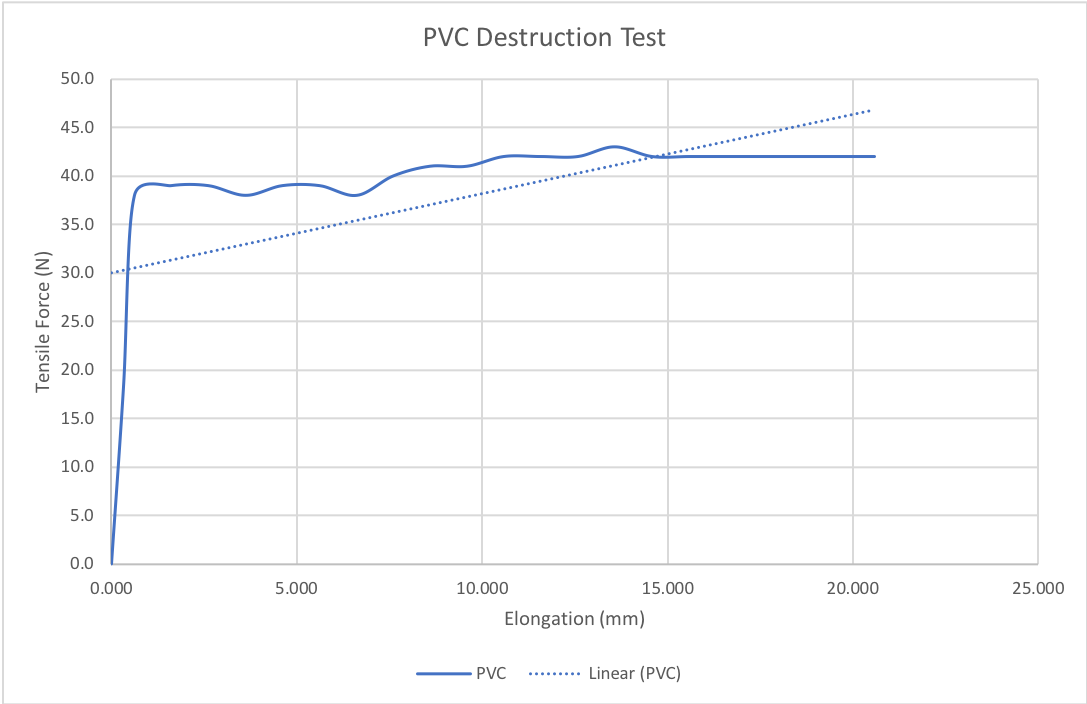
\includegraphics[scale=0.45]{Images/PVC/PVC_Destruction_Trend.png}
\caption{Data collected from PVC destruction.}
\label{PVC Destruction Trend}
\end{figure}

The young's modulus is represented graphical using the trend line function. \\

Hooke's Law;

\begin{equation}
{F = \dfrac{13.570}{14}=0.969mm}
\end{equation}

Tensile Stress;

\begin{equation}
{UTS = \dfrac{0.969}{2.05}=0.473N/mm^2}
\end{equation}

\begin{figure}[H]
\centering
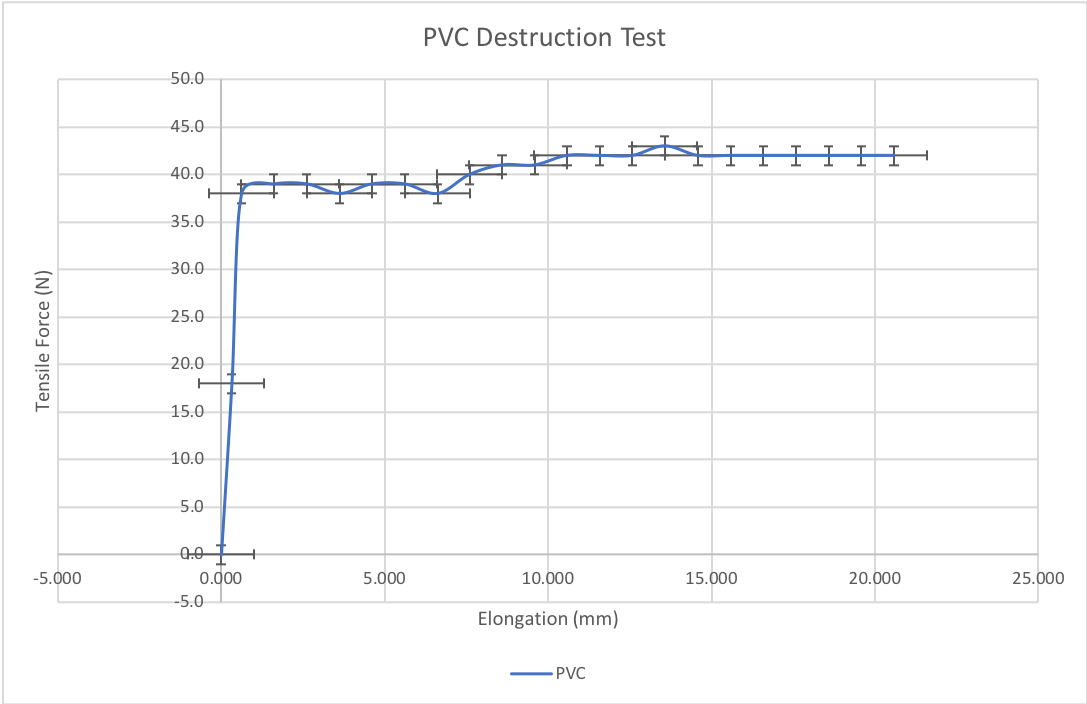
\includegraphics[scale=0.45]{PVC.png/PVC_Destruction_Error.png}
\caption{Data collected from PVC destruction with error.}
\label{PVC Destruction Error}
\end{figure}

\cite{LLR.2-2018}

%-----------------------------------------------------------------------
%	MILD STEEL
%-----------------------------------------------------------------------

\subsection{Mild Steel Sample}
\label{Mild Steel Sample SubSection}

\begin{figure}[H]
\centering
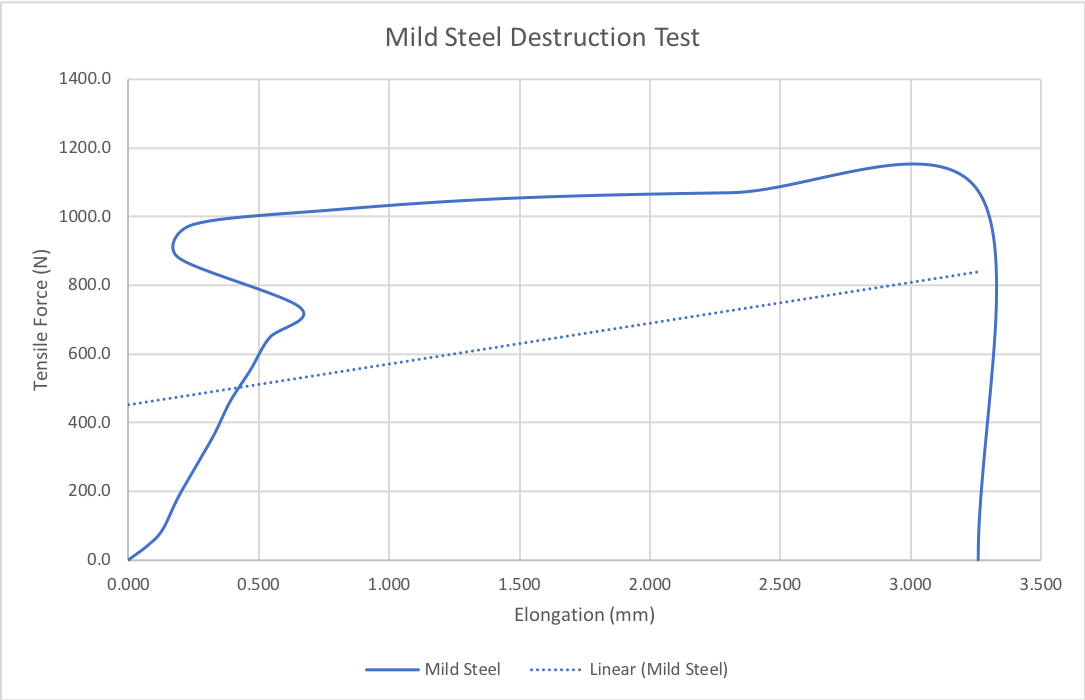
\includegraphics[scale=0.45]{Images/Mild_Steel/MS_Destruction_Trend.png}
\caption{Data collected from Mild Steel destruction.}
\label{Mild Steel Destruction Trend}
\end{figure}

The young's modulus is represented graphical using the trend line function. \\

Hooke's Law;

\begin{equation}
{F = \dfrac{0.800}{11}=0.072mm}
\end{equation}

Tensile Stress;

\begin{equation}
{UTS = \dfrac{0.072}{2.11}=0.034N/mm^2}
\end{equation}

\begin{figure}[H]
\centering
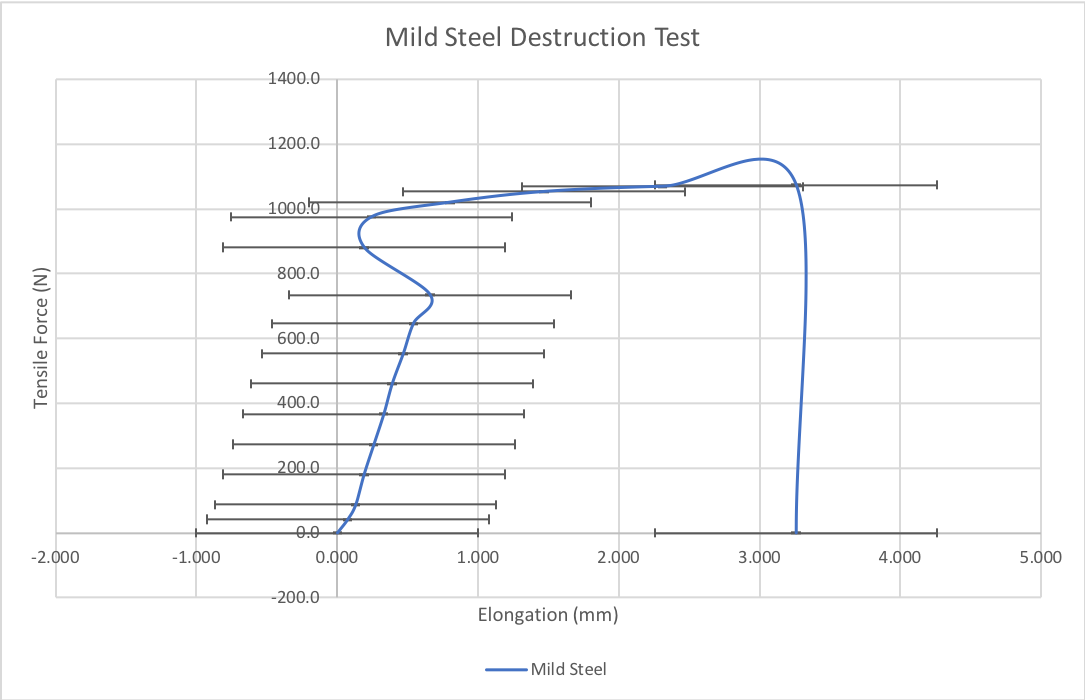
\includegraphics[scale=0.45]{Images/Mild_Steel/MS_Destruction_Error.png}
\caption{Data collected from Mild Steel destruction with error.}
\label{Mild Steel Destruction Error}
\end{figure}

%-----------------------------------------------------------------------
%	ALUMINIUM
%-----------------------------------------------------------------------

\subsection{Aluminium Sample}
\label{Alumnium Sample SubSection}

\begin{figure}[H]
\centering
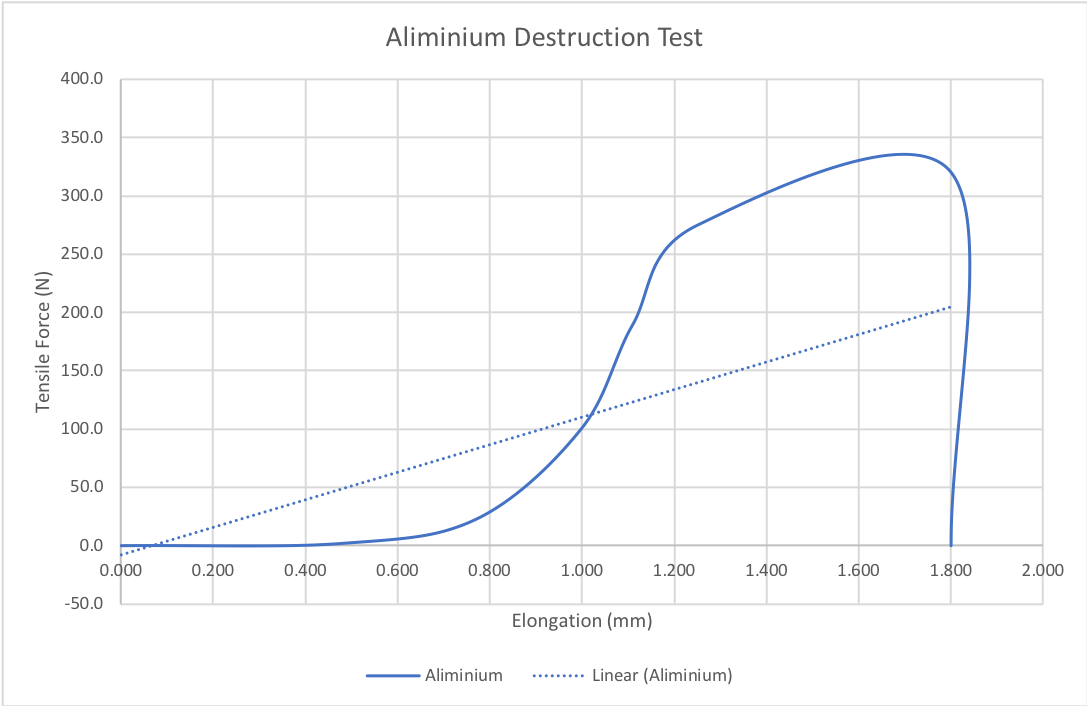
\includegraphics[scale=0.45]{Images/Aluminium/A_Destruction_Trend.png}
\caption{Data collected from Aluminium destruction.}
\label{Aluminium Destruction Trend}
\end{figure}

The young's modulus is represented graphical using the trend line function. \\

Hooke's Law;

\begin{equation}
{F = \dfrac{1.800}{5}=0.360mm}
\end{equation}

Tensile Stress;

\begin{equation}
{UTS = \dfrac{0.360}{2.2}=0.163N/mm^2}
\end{equation}

\begin{figure}[H]
\centering
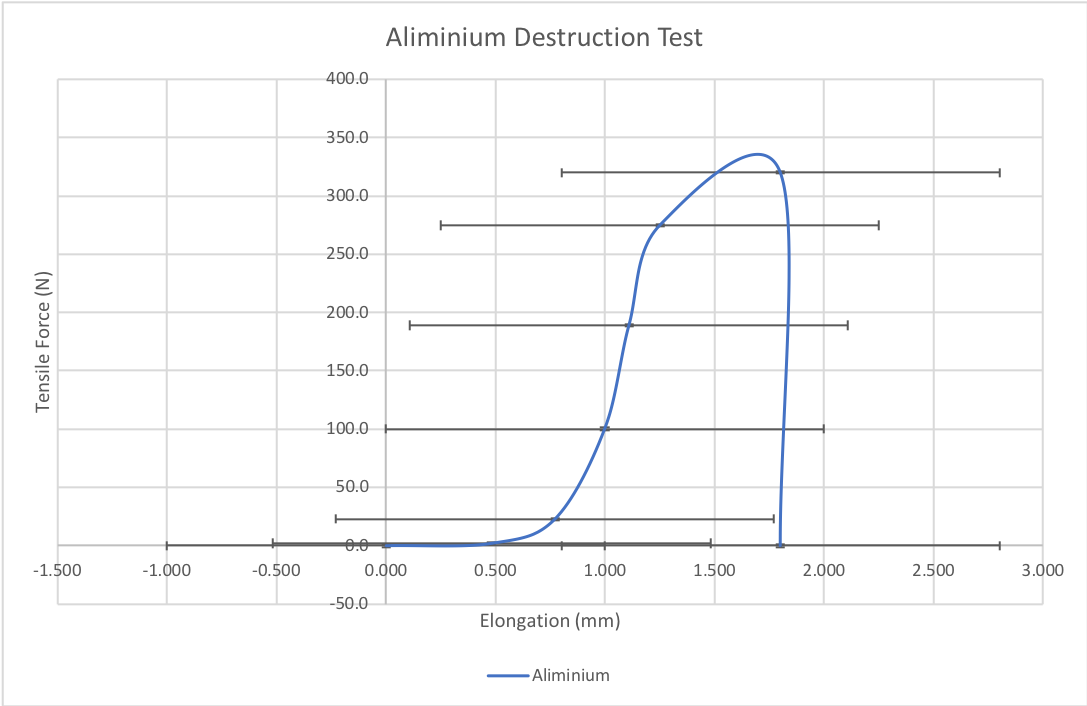
\includegraphics[scale=0.45]{Images/Aluminium/A_Destruction_Error.png}
\caption{Data collected from Aluminium destruction with error.}
\label{Aluminium Destruction Error}
\end{figure}

%-----------------------------------------------------------------------
%	DURALUMIN
%-----------------------------------------------------------------------

\subsection{Duralumin Sample}
\label{Duralumin Sample SubSection}

\begin{figure}[H]
\centering
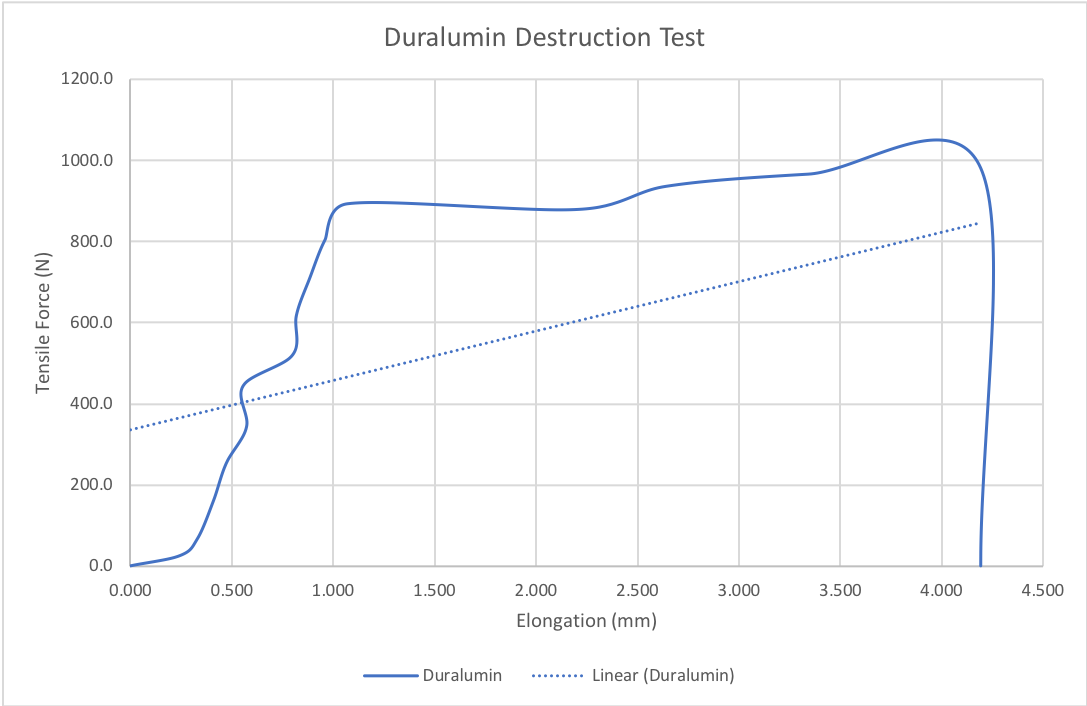
\includegraphics[scale=0.45]{Images/Duralumin/D_Destruction_Trend.png}
\caption{Data collected from Duralumin destruction.}
\label{Duralumin Destruction Trend}
\end{figure}

The young's modulus is represented graphical using the trend line function. \\

Hooke's Law;

\begin{equation}
{F = \dfrac{3.340}{13}=0.257mm}
\end{equation}

Tensile Stress;

\begin{equation}
{UTS = \dfrac{0.257}{2.0}=0.129N/mm^2}
\end{equation}

\begin{figure}[H]
\centering
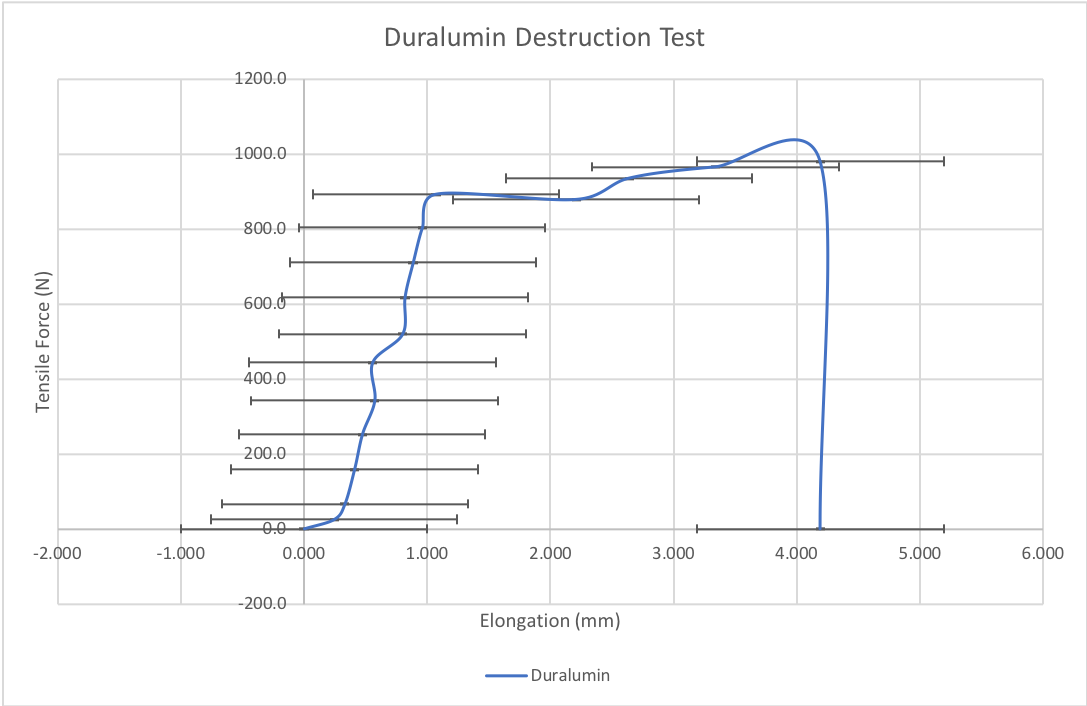
\includegraphics[scale=0.45]{LaTeX Images/Duralumin/D_Destruction_Error.png}
\caption{Data collected from Duralumin destruction with error.}
\label{Duralumin Destruction Error}
\end{figure}

%-----------------------------------------------------------------------
%	ANALYSIS
%-----------------------------------------------------------------------

\section{Analysis}
\label{Analysis Section}

Through analyzing the graphs, it can be said that PVC is a very elastic material making PVC very malleable thus it has a high fracture point compared to the three metals that are have increased hardness making them brittle, thus proving why aircraft would use Duralumin instead of PVC as fuselage. Atomically the metals and PVC are both laid in a lattice structure but due to the elasticity of the PVC it stretches more than the metals as it more brittle and thats why the three metals reaches its fracture points faster than the PVC material. 

%------------------------------------------------------------------------
%	REFERENCES
%------------------------------------------------------------------------

\end{multicols}
\bibliographystyle{plain}
\bibliography{mybib.bib}

%------------------------------------------------------------------------

\end{document}